\documentclass{article}

\usepackage[utf8]{inputenc}
\usepackage[T1]{fontenc}
\usepackage[english]{babel}

\usepackage{float}
\usepackage{amsmath}
\usepackage{graphicx}
\usepackage[colorinlistoftodos]{todonotes}
\usepackage{url}
%pour les informations sur un document compilé en PDF et les liens externes / internes
\usepackage{hyperref}
%pour la mise en page des tableaux
\usepackage{array}
\usepackage{tabularx}
\usepackage{setspace}
%modifier la mise en page de l'abstract
\usepackage{abstract}
%police et mise en page (marges) du document
\usepackage[top=4cm, bottom=4cm, left=4cm, right=4cm]{geometry}
%Pour les galerie d'images
\usepackage{subfig}

%====================== INFORMATION ET REGLES ======================

%rajouter les numérotation pour les \paragraphe et \subparagraphe
\setcounter{secnumdepth}{4}
\setcounter{tocdepth}{4}

\hypersetup{							% Information sur le document
pdfauthor = {Premier Auteur,
			Deuxième Auteur,
			Troisième Auteur,
    		Quatrième Auteur},			% Auteurs
pdftitle = {Nom du Projet -
			Sujet du Projet},			% Titre du document
pdfsubject = {Mémoire de Projet},		% Sujet
pdfkeywords = {Tag1, Tag2, Tag3, ...},	% Mots-clefs
pdfstartview={FitH}}					% ajuste la page à la largueur de l'écran

\begin{document}

%régler l'espacement entre les lignes
\newcommand{\HRule}{\rule{\linewidth}{0.5mm}}

%page de garde
\begin{titlepage}
\begin{center}

\textsc{\LARGE \textbf{\'{E}COLE PRATIQUE DES HAUTES ÉTUDES COMMERCIALES}}\\[0.4cm]

% Upper part of the page. The '~' is needed because only works if a paragraph has started.

\includegraphics[width=0.7\textwidth]{ephec.png}~\\[0.4cm]

\texts{\MEDIUM Avenue du Ciseau, 15}\\
\texts{\MEDIUM 1348 Louvain-La-Neuve}\\[1.5cm]

\textsc{\Large }\\[0.5cm]

% Title
\HRule \\[0.4cm]

{\huge \bfseries Development of a car rental management information system \\[0.4cm] }

\HRule \\[0.5cm]

\textbf{Technical defense}

\vspace{1.cm}

% Author and supervisor
\begin{minipage}{0.4\textwidth}
\begin{flushleft} \large
\emph{Author:}\\
Olivier.D NIYONKURU\\
\end{flushleft}
\end{minipage}
\begin{minipage}{0.4\textwidth}
\begin{flushright} \large
\emph{reporter:} \\
\textsc{Louis VAN DORMAEL}
\end{flushright}
\end{minipage}

\vfill

% Bottom of the page
{\large \today}

\end{center}
\end{titlepage}

%page blanche
\newpage

\section{What}

    Before i proceed to describe how this car reservation system will be developed specifically for my client, let's first take a closer look at what’s exactly the car rental booking software. 
    
    \vspace{0.3cm}
    
    From its name, it’s an innovative booking software designed for cars, motorcycles, boats, or trailer rental companies. It's a secure platform that offers an easy and fast way to smoothly manage car rentals and website reservation systems that makes it an ideal booking software for any rental business.
    
    \vspace{0.3cm}
    
    I will be implementing a custom car reservation solution for my client that maximizes efficiency when it came to automating all car reservation tasks and receiving up-to-date important business statistics.

\section{Problems}

       Personally speaking, i have found myself in a situation trying to get a car over the phone but all lines seemed busy, or maybe i was in a noisy place, where it’s difficult to speak, or vice versa, somewhere i had to be quiet. A tricky task at times.

        \vspace{0.3cm}

       Modern life is busy and dynamic. No wonder people lay their hands on anything that can make things quicker and easier. Car rental software development significantly simplifies the entire process of booking a car. 
        
        \vspace{0.3cm}
        
        My client has some personal vehicles at disposal for people looking to rent a car for a given period. But for the time being my client runs fully his business on his phone(s) by receiving calls of people who want to rent some of his vehicle or those that need a car for a certain period, but does not have the desire or opportunity to buy it.
        
        \vspace{0.3cm}
        
        He wants to go digital and to accept online reservations and manage his fleet with ease. In today’s digital environment, users would rather book cars online instead of calling the rental company to make reservations. If you are running a car rental business, developing a car rental software becomes a must. 
        
        \vspace{0.3cm}
        
        I got in touch with him to implement a well-designed car rental system, not only to accept online reservations and manage his entire fleet, so that his potential customers can reserve available cars online. This car rental system will help run his business smoothly and effectively.

\section{Goals}

  \begin{itemize}
  
	    \item A customer self-service platform to view vehicle              availability in real-time,
	    \item 24/7 accepting online reservations,
	    \item Removing the paper-based processes,
	    \item Detailed analytics and statistics, i.e., the software should deliver an up-to-date analytics to see how his business performs,
	    \item Avoiding risks of overbooking and the factor of          human error,
	    \item The reservations timeline to track the status of the vehicle due for maintenance, for delivery or pick-up, or currently on the road,
	    \item Cuts down on administration processes to improve         business efficiency,
	    \item Making data-driven decisions based on detailed           statistics,
	   \item Feedback system for clients to give reviews and rate the service,
	   \item Provide an estimation of the influx of bookings to prepare for future demands.
	   
	 \end{itemize}

\section{Methodology}

    \textbf{Agile.} I will be meeting (virtually or in person) the client every 2 weeks to discuss my progress and to assess his input. 

\section{Planning}

    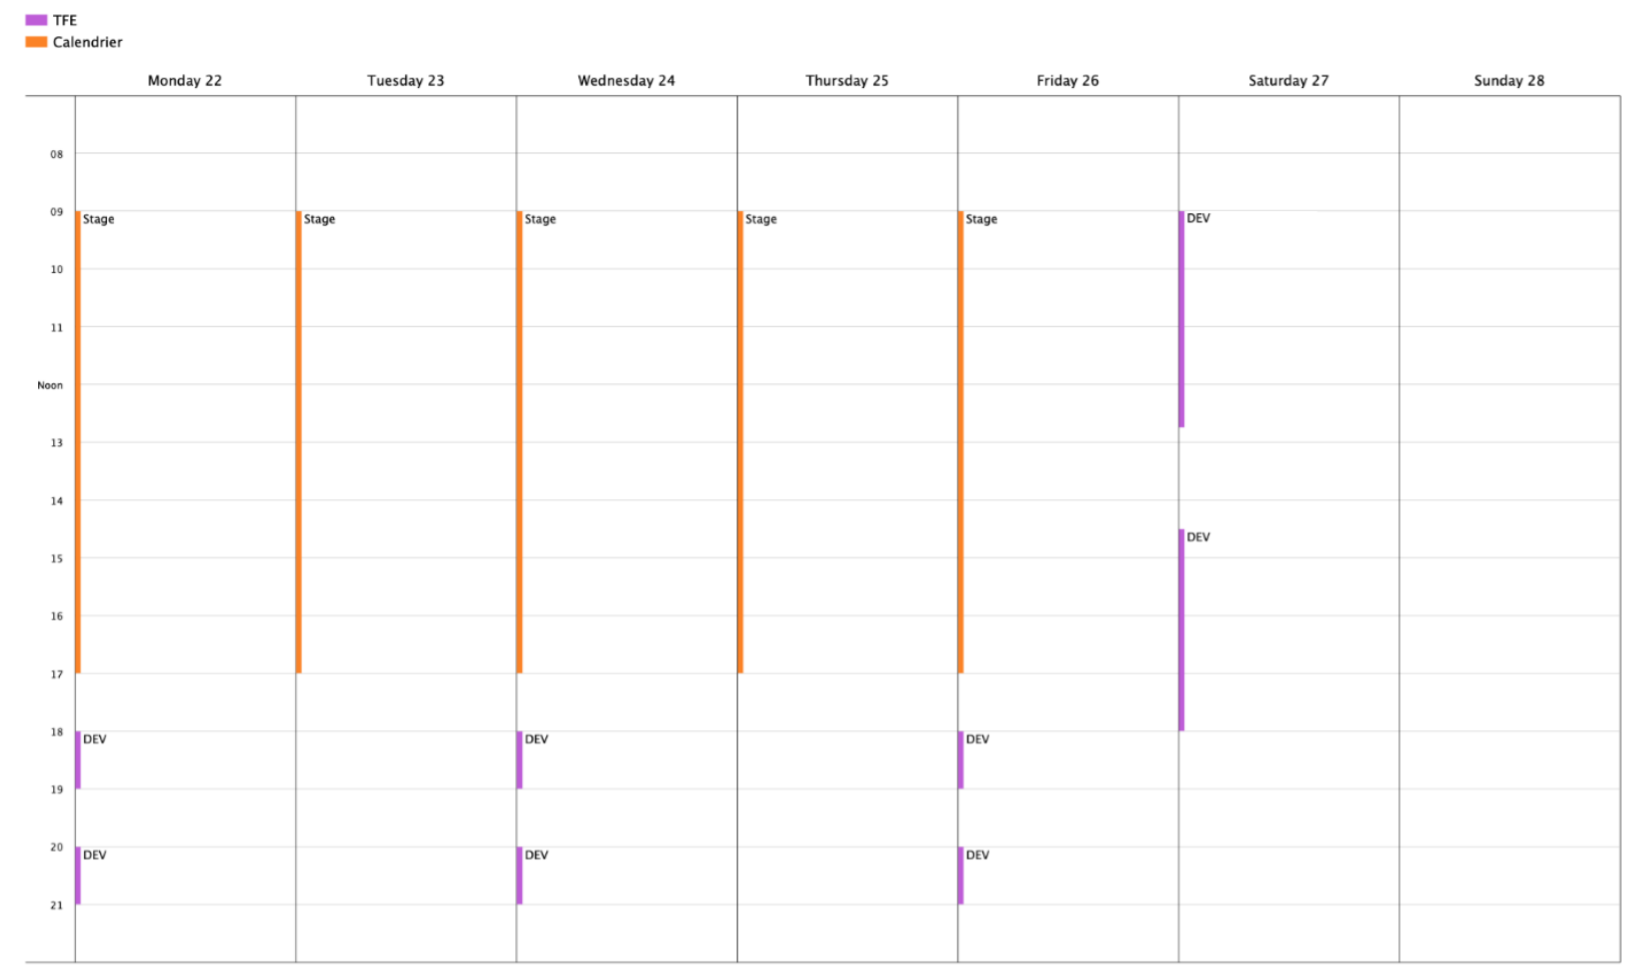
\includegraphics[width=1.2\textwidth]{planning.PNG}~\\[0.2cm]

\pagebreak

\section{Progress}

    \begin{itemize}
        
        \item Contact the client on the technical user stories
        \item E-R diagram
        \item Relational diagram
        \item Use case diagram 
        \item Class diagram
        \item Git repository
        \item Implement the client's user stories in details 
        \item Back-end and front-end setup
        \item Deployment setup 

    \end{itemize}
        
\end{document}
